%%=============================================================================
%% Conclusie
%%=============================================================================
\chapter{Resultaten}%
\label{ch:resultaten}
\section{Onderzoeksopzet}
\vspace{1em}Om de meerwaarde van het ontwikkelde ML-model te beoordelen, werd het vergeleken met drie andere allocatiemethodes: Round-Robin, Greedy Rol-Match en ChatGPT (GPT-4o). Alle methodes ontvingen exact dezelfde invoer: een dataset van 100 taken en 22 werknemers met alle eigenschappen eraan. De evaluatie werd uitgevoerd op zes kwantitatieve metrics die samen de kwaliteit van de verdeling meten.

\vspace{1em}De zes gebruikte metrics zijn:

\vspace{0.5em}Rol-match (\%): het percentage taken dat terechtkomt bij een werknemer met de vereiste rol.

\vspace{0.5em}Skill-overlap (\%): het percentage taken waarbij de toegewezen werknemer minstens één relevante skill bezit.

\vspace{0.5em}Werklastverdeling (std): de standaarddeviatie van het aantal taken per werknemer: een lagere waarde wijst op een eerlijkere spreiding.

\vspace{0.5em}Maximale taaklast: het hoogste aantal taken dat één werknemer ontvangt.

\vspace{0.5em}Minimale taaklast: het laagste aantal taken dat één werknemer ontvangt.

\vspace{0.5em}Overbelasting (\%): het percentage werknemers dat na allocatie een werkdruk van 1,0 of hoger bereikt.

\section{Beschrijving van de methodes}
\vspace{1em}Round-Robin is de meest basische allocatiestrategie: taken worden strikt om de beurt verdeeld over alle werknemers, zonder enige inhoudelijke overweging. Deze methode dient als absolute ondergrens en toont wat er gebeurt bij volledige afwezigheid van intelligentie in het systeem.

Greedy Rol-Match is een regelgebaseerd algoritme dat bij elke taak de minst belaste werknemer met de vereiste rol selecteert. Wanneer geen enkele werknemer die rol bezit, wordt de minst belaste werknemer als fallback gekozen. Het algoritme is eendimensionaal: het optimaliseert uitsluitend voor rol-match en directe werkdruk, zonder rekening te houden met skills, persoonlijkheidskenmerken of ervaringsniveau.

ChatGPT (GPT-4o) ontving een gestructureerde prompt met alle werknemers- en taakgegevens en werd gevraagd elke taak te verdelen op basis van rol, werkdruk, skills en moeilijkheidsgraad. In tegenstelling tot de twee vorige methodes maakt ChatGPT gebruik van een model dat meerdere criteria tegelijk kan afwegen.

Het ML-model is een Random Forest classifier die getraind werd op een samengestelde score die vier criteria combineert: rol-match, persona-fit (op basis van persoonlijkheidskenmerken), werkdruk en het huidige taakaantal. Het model leert patronen in welke combinaties van werknemers en taken het beste zijn en past deze kennis toe bij nieuwe toewijzingen.

\begin{listing}
  \begin{minted}{python}
        def metrics(assignments):
        role_match, skill_hits = 0, 0
        workload = {e["name"]: e.get("workload", 0.0) for e in employees}
        counts   = Counter()
        for task, emp in assignments:
        counts[emp["name"]] += 1
        workload[emp["name"]] = min(1.0, workload[emp["name"]] + 0.1)
        req = task["required_role"]
        if req == emp["role"] or (req == "Senior Developer" and emp["role"] == "Developer"):
        role_match += 1
        task_text = (task["task"] + " " + task.get("type","")).lower()
        if any(s.lower() in task_text for s in emp.get("skills",[])):
        skill_hits += 1
        n = len(assignments)
        c = [counts.get(e["name"], 0) for e in employees]
        overload = sum(1 for w in workload.values() if w >= 1.0)
        return {
            "Rol-match %":            round(100 * role_match / n, 1),
            "Skill-overlap %":        round(100 * skill_hits / n, 1),
            "Werklastverdeling std":  round(statistics.stdev(c), 2),
            "Max taken (1 persoon)":  max(c),
            "Min taken (1 persoon)":  min(c),
            "Overbelasting %":        round(100 * overload / len(employees), 1),
        }
      \end{minted}
  \caption[Stukje van het evaluatiescript]{Stukje van het evaluatiescript waarin de code staat voor de metrics.}
\end{listing}

\begin{table}
    \centering
    \begin{tabular}{lrrrr}
        \toprule
        \textbf{Metric} & \textbf{Round-Robin} & \textbf{Greedy} & \textbf{ChatGPT} & \textbf{ML-model} \\
        \midrule
        Rol-match (\%)            & 21{,}0 & \textbf{100{,}0} & \textbf{100{,}0} & 46{,}0 \\
        Skill-overlap (\%)        & 0{,}0  & 3{,}0            & \textbf{11{,}0}  & 2{,}0  \\
        Werklastverdeling (std)   & \textbf{0{,}51} & 3{,}13  & 3{,}35           & 1{,}37 \\
        Max.\ taken (1 persoon)   & \textbf{5}      & 10      & 13               & 7      \\
        Min.\ taken (1 persoon)   & \textbf{4}      & 0       & 0                & 3      \\
        Overbelasting (\%)        & 59{,}1 & 50{,}0           & 54{,}5           & \textbf{54{,}5} \\
        \bottomrule
    \end{tabular}
    \caption[Vergelijking taakallocatiemethodes]{\label{tab:vergelijking}Vergelijking van vier taakallocatiemethodes op zes metrics. Vetgedrukt = beste score per metric.}
\end{table}

\begin{figure}
  \centering
  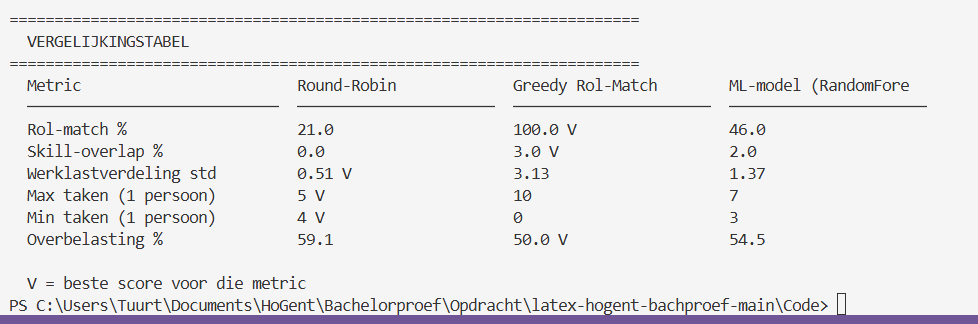
\includegraphics[width=0.8\textwidth]{../graphics/screenshot010.png}
  \caption[Uitvoer evaluatiescript.py]{\label{fig:screenshot010}De uitvoer van het evaluatiescript}
\end{figure}

\section{Analyse per methode}
\vspace{1em}Round-Robin scoort uitsluitend sterk op de verdelingsmetrics: elke werknemer ontvangt 4 à 5 taken, wat resulteert in de laagste standaarddeviatie (0,51) en de kleinste spreiding tussen minimum en maximum taaklast. Dit is eerder niet de beste oplossing want slechts 21\% van de taken wordt toegewezen aan iemand met de vereiste rol en er is geen enkele skill-overlap. In een reële werkomgeving zou dit systeem volledig onbruikbaar zijn, omdat bijvoorbeeld beveiligingstaken aan developers worden toebedeeld en IT-ondersteuning aan systeembeheerders.

Greedy Rol-Match lost het rolprobleem volledig op: 100\% van de taken belandt bij de juiste rol. Het knelpunt is wel dat het een ernstig ongelijke verdeling heeft: de standaarddeviatie loopt op tot 3,13, 1 werknemer ontvangt maximaal 10 taken, terwijl vier andere werknemers: Sophie Dubois, Laura De Wilde, Elena Petrova en Mark De Vries geen enkele taak ontvangen. Een perfecte rol-match gecombineerd met zulke extreme taakverdeling is in de praktijk niet werkbaar.

ChatGPT (GPT-4o) behaalt sterke scores: 100\% rol-match en de hoogste skill-overlap van alle methodes (11\%). Dit toont aan dat het model verder kijkt dan enkel de rolbenaming en ook de skills van werknemers meeneemt in zijn redenering. Zo worden Python-ontwikkelaars bij data-taken ingezet en security-specialisten bij beveiligingstaken, wat verder gaat dan puur rolgebaseerde matching. Echter schiet ChatGPT tekort op verdelingsniveau: de standaarddeviatie is met 3,35 de hoogste van alle methodes, één werknemer:  Ahmed Benali ontvangt maar liefst 13 taken, terwijl Laura De Wilde en Mark De Vries geen enkele taak krijgen. ChatGPT optimaliseert voor de kwaliteit van individuele toewijzingen, maar vergeet de gehele werklastverdeling goed in kaart te brengen.

Het ML-model neemt een tussenpositie in. De rol-match van 46\% ligt beduidend lager dan die van Greedy en ChatGPT, maar dit is het gevolg van een bewuste afweging waarbij beginwerkdruk en persoonlijkheidsfit worden meegewogen naast de rol. Werknemers met een hoge beginwerkdruk (0,9) worden actief ontzien, ook wanneer zij de vereiste rol bezitten. Het resultaat is een werklastverdeling met standaarddeviatie 1,37, wat beduidend eerlijker is dan zowel Greedy als ChatGPT, terwijl niemand zonder taken blijft (minimum = 3) en niemand meer dan 7 taken ontvangt. De overbelasting (54,5\%) is gelijk aan die van ChatGPT, maar bereikt dat resultaat met een gelijkmatigere spreiding over het volledige team.

\section{Besluit}
\vspace{1em}De vier methodes vertegenwoordigen elk een andere prioritering in het allocatieprobleem. Round-Robin maximaliseert eerlijkheid maar negeert inhoud volledig. Greedy en ChatGPT maximaliseren inhoudelijke kwaliteit, waarbij ChatGPT dankzij skill-bewustzijn zelfs verder gaat dan Greedy, maar beide creëren onaanvaardbare taakverdeling bij een minderheid van werknemers. Het ML-model is de enige methode die beide dimensies systematisch balanceert: het levert een redelijke inhoudelijke kwaliteit terwijl het de werklast evenwichtig spreidt over het volledige team.

Dit onderscheid is in de praktijk van groot belang. Een allocatiesysteem dat technisch correcte toewijzingen maakt maar consequent dezelfde werknemers overbelast, is op de middellange termijn niet houdbaar. Het ML-model lost dit op door werkdruk en persona-fit als expliciete criteria in het leerproces op te nemen, wat resulteert in een allocatie die duurzamer is voor het welzijn van het team als geheel. De sterke interne modelkwaliteit: recall van 1,00, ROC-AUC van 0,98 en stabiele kruisvalidatiescores bevestigt dat het model betrouwbaar presteert, al blijft de afhankelijkheid van synthetische trainingsdata een aandachtspunt voor verdere ontwikkeling.

%--------------------------------------------------------------------------------------
\chapter{Conclusie}%
\label{ch:conclusie}
% TODO: Trek een duidelijke conclusie, in de vorm van een antwoord op de
% onderzoeksvra(a)g(en). Wat was jouw bijdrage aan het onderzoeksdomein en
% hoe biedt dit meerwaarde aan het vakgebied/doelgroep? 
% Reflecteer kritisch over het resultaat. In Engelse teksten wordt deze sectie
% ``Discussion'' genoemd. Had je deze uitkomst verwacht? Zijn er zaken die nog
% niet duidelijk zijn?
% Heeft het onderzoek geleid tot nieuwe vragen die uitnodigen tot verder 
%onderzoek?
\vspace{1em}

